%%%%%%%%%%%%%%%%%%%%%%%%%%%%%%%%%%%%%%%%%%%%%%%%
%
%  CHAPTER 2: Analog-to-Digital Converters and DSMs
%
%%%%%%%%%%%%%%%%%%%%%%%%%%%%%%%%%%%%%%%%%%%%%%%%

%%%%%%%%%%%%%%%%%%%%%%%%%%%%%%%%%%%%%%%%%%%%%%%%
%%% Section 2.1 - Introduction
%%%%%%%%%%%%%%%%%%%%%%%%%%%%%%%%%%%%%%%%%%%%%%%%
% \section{Introduction}
Analog-to-digital converters (ADCs) are systems which convert continuous-time, continuous
amplitude, or analog, signals into discrete-time, discrete amplitude, or digital signals.
Typically, an ADC converts an analog signal, $x_a(t)$, defined over a continuous finite
interval, $R$, into a digital signal, $x(n)$, defined over a discrete number, $L$, of
values which span the interval $R$. The number, $L$, of discrete values that an ADC can
produce is referred to as the ADC's resolution. Because most ADCs interface with binary
electronic systems, an ADC's resolution is typically a power of 2; that is, $L=2^B$ where
$B$ is an integer representing the binary bit-width of the ADC interface. Thus, ADC
resolution is often expressed in terms of the number, $B$, of bits and not the number,
$L$, of available quantization levels.

\sloppy
For linear ADCs, each of the $2^B$ quantization levels are equidistant over the signal
span $R$. For such ADCs, the quantization step size, $\Delta$, or distance between
adjacent quantization levels is expressed as $\Delta=R/2^B$ where $R$ corresponds to the
input signal span as defined above. For example, consider an analog input, $x_a(t)$, which
has a signal span from -1 to 1; that is, consider an analog input, $x_a(t)$, where
$$-1\leq
x_a(t) \leq 1$$ which has a signal span, $R$, where $R=2$. For a 2-bit system, the signal
span, $R$, is divided into $2^2$ equidistant levels where the quantization step size,
$\Delta$, is $$\Delta=\frac{R}{2^B}=\frac{2}{2^2}=0.5\text{.}$$ This example is
illustrated in Figure \ref{fig:2_bit_quant} for $x_a(t)=\cos(2\pi 1000 t)$, $x_a(n
T_s)=\cos(\pi n/32)$ for $T_s=1/64\pi 1000$, and $x(n)=\mathcal{Q}\left[x_a(n
T_s)\right]$ where $T_s$ is the sampling period in time per sample and 
$\mathcal{Q}[\cdot]$ is the transformation that quantizes the continuous amplitude,
discrete-time signal, $x_a(nT_s)$, by rounding the amplitude to the nearest quantization
level.
%-------------------
\begin{figure}[htbp]
 \centering
 \includegraphics[width=0.8\textwidth]{./matlab_figures/2_bit_intro}
 \caption{2-Bit Quantization}
 \label{fig:2_bit_quant}
\end{figure}
%-------------------

The difference, $x_a(n T_s)-x(n)$, is commonly referred to as the quantization error and
is often characterized as quantization noise in the ADC's output. As shown in Figure
\ref{fig:2_bit_quant}, the digital signal, $x(n)$, is different than both the
analog input signal, $x_a(t)$, and the discrete-time, continuous amplitude signal, 
$x_a(n T_s)$. As the number, $B$, of bits increases, the quantization error, or 
quantization noise, typically decreases. Thus, an ADC's quantization noise is typically a
function of the number, $B$, of quantization bits. In practice, however, ADC levels are
not equally spaced; that is, $\Delta$ varies slightly over the interval $R$. This
non-uniformity in level spacing creates distortion which is also often characterized as
noise in the ADC output. Non-uniform level spacing along with other non-idealities such as
improper input signal conditioning, system thermal noise, and sample clock jitter, limit
an ADC's effective resolution to less than the ideal. As a result, an ADC's effective
resolution is often determined from the ADC's output signal-to-noise ratio (SNR) or
dynamic range (DR) which are performance metrics that are  independent of the ADC's native
architecture.

SNR is defined as the ratio of output signal power to output noise power which contains
power from quantization error and other ADC non-idealities. Dynamic range is defined as
the ratio of the maximum to the minimum detectable signal levels. DR differs from SNR when
the noise floor is not perfectly flat; i.e., noise power in localized frequency regions is
greater than the average noise power. The effects of DR further limit the practical
performance of ADCs. As such, an ADC's effective resolution is often calculated from
the ADC's SNR and DR. The effective resolution is referred to as the ADC's effective
number of bits (ENOB) where ENOB is defined as the achievable ADC resolution when its
non-ideal ADC characteristics are considered.

$\Delta\Sigma$ modulators are ADCs which achieve high SNRs and large DRs by using a
feedback loop filter to attenuate the quantization noise in the frequency band of
interest while passing the input signal to the output. The transfer function describing
the loop filter that attenuates the quantization noise is referred to as the noise
transfer function (NTF). Similarly, the transfer function describing the loop filter that
passes the input signal to the output is referred to as the signal transfer function
(STF).  For example, the NTF for lowpass $\Delta\Sigma$ modulators is designed as a
highpass filter so that the noise energy is attenuated within the low-frequency signal
band. The STF for lowpass $\Delta\Sigma$ modulators is designed as a lowpass
filter so that the input signals within the low-frequency signal band are not attenuated.
In addition, the lowpass characteristics of the STF can also act as an anti-aliasing
filter. As such, the output of a lowpass $\Delta\Sigma$ modulator can be modeled as the
sum of a noise source that is highpass filtered by the NTF and an input signal that is
lowpass filtered by the STF.

 $\Delta\Sigma$ modulator NTFs and STFs are typically designed and implemented  as either
discrete or analog linear recursive filters. As such, a $\Delta\Sigma$ modulator's NTF and
STF can be designed using traditional filters such as Chebyshev or Butterworth filters.
However, these methods are not easily adaptable to the atypical frequency response
characteristics commonly required by many $\Delta\Sigma$ modulators. Historically,
numerical optimization methods have been applied to the optimal design of linear recursive
filters with good success
\cite{rabiner_linear_1974}\cite{chen_design_1990}\cite{cortelazzo_simultaneous_1984}. As
such, design techniques which rely heavily on numerical optimization methods can be used
to optimize $\Delta\Sigma$ modulator system design. Some numerical filter design
programs include other electronic design automation (EDA) tools which automate much of the
design process. For example, the Delta Sigma Toolbox for
MATLAB\textsuperscript{\textregistered} provides an integrated set of discrete-time
$\Delta\Sigma$ modulator design, simulation, and synthesis utilities
\cite{schreier_understanding_2004}. However, this thesis will show that the design method
in the Delta Sigma toolbox offers only marginal improvement over traditional Chebyshev or
Butterworth polynomial based filter design methods.

In this thesis, a global numerical optimization algorithm, called the hybrid orthogonal
genetic (HOG) algorithm, is developed which can determine the optimal design of both
discrete and analog linear recursive filters. In this thesis, the HOG algorithm is used to
optimize the performance of $\Delta\Sigma$ modulator's NTFs and STFs by maximizing
the in-band SNR and DR.

%%%%%%%%%%%%%%%%%%%%%%%%%%%%%%%%%%%%%%%%%%%%%%%%
%%% Section 2.2 - ADC Operational Theory
%%%%%%%%%%%%%%%%%%%%%%%%%%%%%%%%%%%%%%%%%%%%%%%%
\section{Operational Theory}
Figure \ref{fig:basic_adc} shows a basic mathematical model of an ADC. As illustrated,
ADCs can be modeled as a sample-and-hold (S/H) circuit in series with a quantizer and
binary encoder. The sample-and-hold circuit samples the analog input signal at discrete
times where the sample-and-hold process is defined as the process of capturing  the
input signal's amplitude at the sample times, $n T_s$, where $n\in I$, and holding it over
the sampling period, $T_s$. The quantizer then approximates the sampled signal's
amplitude, $x_a(n T_s)$, by converting it to one of the ADC's $L$ quantization levels
which are uniformly spaced by the distance $\Delta$ for a linear ADC. Finally, the
binary encoder converts the digital signal, $x(n)$, into a $B$-bit binary code word.
%-------------------
\begin{figure}[htbp]
 \centering
 \includegraphics{./final_figures/basic_ADC.eps}
 \caption{Basic ADC Block Diagram}
 \label{fig:basic_adc}
\end{figure}
%-------------------

%%%%%%%%%%%%%%%%%%%%%%%%%%%%%%%%%%%%%%%%%%%%%%%%
%%% 2.2.1: Sampling
%%%%%%%%%%%%%%%%%%%%%%%%%%%%%%%%%%%%%%%%%%%%%%%%
\subsection{Sampling}
The Shannon-Nyquist sampling theorem states that an analog signal must be sampled at a
rate that is at least twice its bandwidth for the analog signal to be reconstructed from
its samples. Specifically, the Shannon-Nyquist sampling theorem states that if an analog
signal, $x_{a}(t)$, is strictly bandlimited such that its Fourier transform, $X_a(f)$, has
the property that $$X_{a}(f) = 0 \quad\lvert f\lvert > f_{0}\text{,}$$ where $f$ is the
instantaneous frequency in cycles per second or Hertz (Hz) and $f_0$ is a fixed frequency,
then $x_a(t)$ can be recovered from its samples, $x_a(n T_s)$, if 
%---------------
\begin{equation}\label{eq:nyquist}
 T_s\leq\frac{1}{2f_{0}}
\end{equation}
%---------------
where $T_s$ is the sampling period in time per sample. The frequency, $f_0$, is referred
to as the Nyquist frequency and the frequency, $2f_{0}$, is referred to as the Nyquist
rate. Converters which sample the input at or near $2f_0$ samples per second  are referred
to as Nyquist rate converters. Common Nyquist rate converter architectures include flash,
dual-slope, successive approximation (SAR), and pipelined converters
\cite{wikipedia_contributors_analog-to-digital_2007}.


%%%%%%%%%%%%%%%%%%%%%%%%%%%%%%%%%%%%%%%%%%%%
%%% 2.2.2 Quantization
%%%%%%%%%%%%%%%%%%%%%%%%%%%%%%%%%%%%%%%%%%%%
\subsection{Quantization}
In this thesis, the quantization transformation, denoted $\mathcal{Q}[\cdot]$, is a
nonlinear transformation which approximates a discrete-time, continuous amplitude
signal by a digital signal that has a finite number of fixed quantization levels. To
illustrate, consider an analog signal, $x_a(t)$, and its corresponding quantized 
signal $x(n)$ where $x(n)=\mathcal{Q}\left[x_a(nT_s)\right]$. If $x(n)$ is a
$B$-bit quantized signal, then the number of quantization
levels, $L$, can be expressed as
%---------------
\begin{equation}\label{eq:quantization_bits}
 L=2^B\text{.}
\end{equation}
%---------------
If the quantized signal, $x(n)$, is bounded such that
%---------------
\begin{equation}\label{eq:quant_magnitude}
\bigl|x(n)\bigr|\leq X_m
\end{equation}
%---------------
where $X_m$ represents the quantizer's maximum input amplitude without saturation, the
quantization interval or step size, $\Delta$, defined as the distance between any two
adjacent quantization levels, can then be expressed as 
%---------------
\begin{equation}\label{eq:quantization_delta}
 \Delta=\frac{X_m}{2^{B-1}}\text{.}
\end{equation}
%---------------

The difference between the discrete-time, continuous amplitude signal, $x_a(nT_s)$,
and the digital signal, $x(n)$, is referred to as the quantization error, $e(n)$. As such,
the quantizer's output, $x(n)$, can be expressed as the sum of the sampled analog
signal, $x_a(n T_s)$, and the quantization error, $e(n)$; that is,
%---------------
\begin{equation}\label{eq:quantizer_output}
x(n)=\mathcal{Q}\bigl[x_a(n T_s)\bigr]=x_a(n T_s)+e(n)
\end{equation}
%---------------
where $\mathcal{Q}[\cdot] $ represents the nonlinear quantization transformation. If a
rounding
quantizer is implemented and it is assumed that:
%---------------
\begin{itemize}
 \item $e(n)$ is a stationary random process
 \item $e(n)$ is uncorrelated with the quantizer's input
 \item $e(n)$ is a white noise process; i.e. it's samples are uncorrelated
 \item $e(n)$ has a probability density that is uniform over the quantization
error range $\bigl[-\Delta/2,\Delta/2\bigr]$
\end{itemize}
%---------------
then the quantizer shown in Figure \ref{fig:linear_quantizer_model}(a) can be modeled by
the linear system shown in Figure \ref{fig:linear_quantizer_model}(b)\cite{
gray_quantization_1990}\cite{ oppenheim_discrete-time_1999}. Using this linear
quantizer model greatly reduces the complexity associated with ADC analysis at the expense
of modeling accuracy. However, it has been shown that for rapidly varying input signals
and small quantization intervals or $\Delta$'s, the results obtained from this linear
noise model are sufficient for most
calculations\cite{oppenheim_discrete-time_1999}\cite{hayes_schaums_1998}.
%-------------------
\begin{figure}[htbp]
 \centering
 \includegraphics*[clip,viewport=0 0 330
150]{./final_figures/linear_quantizer_model.eps}
 \captionsetup{justification=centering} 
 \caption[]{Linear Quantizer Model\\(a) Nonlinear Quantizer (b) Linear
Quantizer Model}
 \label{fig:linear_quantizer_model}
\end{figure}
%-------------------

%%%%%%%%%%%%%%%%%%%%%%%%%%%%%%%%%%%%%%%%%%%%
%%% 2.3 ADC Performance Metrics
%%%%%%%%%%%%%%%%%%%%%%%%%%%%%%%%%%%%%%%%%%%%
\section{Performance Metrics}
An ADC's performance is often described in terms of SNR and DR where both
metrics compare the relative output signal power to the output noise power. Because
deterministic signals and stochastic noise are modeled differently, their respective
powers are calculated using different techniques. For deterministic signals,
power is calculated analytically from the available signal information. For stochastic
signals, power is calculated in terms of the statistical characteristics which define the
signal.

%%%%%%%%%%%%%%%%%%%%%%%%%%%%%%%%%%%%%%%%%%%%%%%%
%%% 2.3.1: Signal and Noise Power
%%%%%%%%%%%%%%%%%%%%%%%%%%%%%%%%%%%%%%%%%%%%%%%%
\subsection{Signal and Noise Power}
The mean or expectation of a continuous random process, $x(t)$, is defined as
 %----------------------
\begin{equation}\label{eq:cont_ensemble_average}
 E\bigl[x(t)\bigr] = \int_{-\infty}^{\infty}{x(t) p_x\bigl(x\left(t\right)\bigr)dx(t)}
\end{equation}
%----------------------
where $p_x\bigl(x\left(t\right)\bigr)$ is the probability density function of $x(t)$.
Similarly, the mean or expectation of a discrete random process, $x(n)$, is defined as
 %----------------------
\begin{equation}\label{eq:discrete_ensemble_average}
 E\bigl[x(n)\bigr] = \sum_{k=1}^{N}{x_k(n)P_{x_k(n)}\bigl(x_k(n)\bigr)}
\end{equation}
%----------------------
where $\{x_k(n): k=1,\cdots,N\}$ is the range of $x(n)$, and
$P_{x_k(n)}\bigl(x_k(n)\bigr)$ is the probability mass function of $x(n)$. Equations
\eqref{eq:cont_ensemble_average} and \eqref{eq:discrete_ensemble_average} are
referred to as the ensemble or state averages of a random process.

The variance, $\sigma_x^2$, of a random process, $x$, is defined as
 %----------------------
\begin{equation}\label{eq:variance}
\sigma_x^2=E\Bigl[\bigl(x-E[x]\bigr)^2\Bigr]
\end{equation}
%----------------------
which can be expressed as 
 %----------------------
\begin{equation}\label{eq:expectation_proof}
\begin{split}
\sigma_x^2& =E\Bigl[\bigl(x-E[x]\bigr)^2\Bigr]\\
& = E\bigl[x^2 - 2xE[x]+E^2[x]\bigr]\\
& = E\left[x^2\right] - E^2[x]\text{.}
\end{split}
\end{equation}
%----------------------
For a zero mean random process, \eqref{eq:expectation_proof} reduces to
 %----------------------
\begin{equation}\label{eq:zero_mean_variance}
\sigma_x^2=E\left[x^2\right]\text{.}
\end{equation}
%----------------------

Calculating the expectation or variance of a random process requires its probability
density or probability mass function. In practice, the probability densities or
probability mass functions for the random variables of a random process are not
necessarily well defined. However, if a random process is said to be ergodic, then the
random process' ensemble average is equivalent to
its time average, and time averages can be used to estimate the random process' mean and
variance\cite{papoulis_probability_1984}\cite{lathi_modern_1998}.

For a continuous-time random process, $x(t)$, the time average, $\mu_{x(t)}$, of $x(t)$ is
defined as 
%----------------------
\begin{equation}\label{eq:cont_time_average}
 \mu_{x(t)}=\displaystyle\lim_{T \to \infty}{\frac{1}{2T}}\int_{-T}^{T}{x(\tau)d\tau}.
\end{equation}
%----------------------
Similarly, for a discrete-time random process, $x(n)$, the time average, $\mu_{x(n)}$,
of $x(n)$ is defined as 
%----------------------
\begin{equation}\label{eq:discrete_time_average}
 \mu_{x(n)}=\displaystyle\lim_{N \to \infty}{\frac{1}{2N+1}}\sum_{k=-N}^{N}{x(k)}.
\end{equation}
%----------------------

Thus, if a zero mean, continuous-time  random process, $x(t)$, is ergodic, the variance,
$\sigma_{x(t)}^2$, of $x(t)$ can be represented in terms of its time average,
$\mu_{x^2(t)}$, as
 %----------------------
\begin{equation}\label{eq:cont_time_variance}
\sigma_{x(t)}^2=E\left[x^2(t)\right]=\mu_{x^2(t)}=\lim_{T \to \infty}
\frac{1}{2T}\int_{-T}^{T}{x^2(\tau)d\tau}\text{.}
\end{equation}
%----------------------
Similarly, if a zero mean, discrete-time random process, $x(n)$, is ergodic, the variance,
$\sigma^2_{x(n)}$, of $x(n)$ can be represented in terms of its time average,
$\mu_{x^2(t)}$, as
 %----------------------
\begin{equation}\label{eq:discrete_time_variance}
\sigma^2_{x(n)}=E\left[x^2(n)\right]=\mu_{x^2(t)}=\lim_{N \to \infty}
\frac{1}{2N+1}\sum_{k=-N}^{N}{x^2(k)}\text{.}
\end{equation}
%----------------------

The power, $P_{x(n)}$, for a deterministic discrete-time signal, $x(n)$, can be calculated
as
%----------------------
\begin{equation}\label{eq:signal_power}
P_{x(n)} =\lim_{N \to
\infty}\frac{1}{2N+1}\sum_{k=-\infty}^{\infty}{x^2(k)}
\end{equation}
%----------------------
which is identical to \eqref{eq:discrete_time_variance}. Therefore, for a zero mean
random signal, $x(n)$, $P_{x(n)}=\sigma^2_{x(n)}$. In practice, SNR and DR are estimated
using
a finite length sequence. Thus, for a signal of length $2N+1$, the average signal
power, $P_{x(n)[-N,N]}$, is
given as
%----------------------
\begin{equation}\label{eq:average_signal_power}
 P_{x(n)[-N,N]} =\frac{1}{2N+1}\sum_{k=-N}^{N}{x^2(k)}\text{.}
\end{equation}
%----------------------
Because \eqref{eq:discrete_time_variance} and \eqref{eq:average_signal_power} are
identical for finite length signals, $$P_{x(n)[-N,N]}=P_{x(n)}=\sigma^2_{x(n)}$$ for zero
mean signals of length $2N+1$.

Recall that a quantizer's output, $x(n)$, which is also the ADC's output,
can be modeled linearly as the sum of the continuous amplitude, discrete-time signal,
$x_a(n T_s)$, and the quantization error, $e(n)$, as given in \eqref{eq:quantizer_output}.
Because $x_a(n T_s)$ and $e(n)$ are assumed to be uncorrelated and $e(n)$ is modeled as a
zero mean random process, the output power, $P_{x(n)}$, of $x(n)$ can be expressed as
%----------------------
\begin{equation}\label{eq:output_power}
\begin{split}
P_{x(n)}& = E\left[x^2(n)\right]\\
& = E\Bigl[\bigl(x_a(nT_s) + e(n)\bigr)^2\Big]\\
& = E\bigl[x^2_a(nT_s)\bigr]+2E\bigl[x_a(nT_s)e(n)\bigr]+E\bigl[e^2(n)\bigr]\\
& =
E\bigl[x^2_a(nT_s)\bigr]+2E\bigl[x_a(nT_s)\bigr]E\bigl[e(n)\bigr]+E\bigl[e^2(n)\bigr]\\
& = E\left[x_a^2(n T_s)\right]+E\left[e^2(n)\right]\\
& =P_{x_a(n T_s)} + P_{e(n)} 
\end{split}
\end{equation}
%----------------------
where $P_{x_a(n T_s)}$ and $P_{e(n)}$ correspond to the output signal power and output
noise power, respectively. Because the quantizer's input, $x_a(nT_s)$, is
typically modeled deterministically, its average signal power, $P_{x_a(n T_s)}$, can 
be given as
%----------------------
\begin{equation}\label{eq:average_quantizer_input_power}
 P_{x_a(n T_s)} = \lim_{N \to\infty}\frac{1}{2N+1}\sum_{n=-N}^{N}x_a^2(nT_s)
\end{equation}
%----------------------
or for finite length signals of length $2N+1$ or periodic signals that have a period of 
$2N+1$ as
%----------------------
\begin{equation}\label{eq:average_quantizer_input_power_finite_length}
 P_{x_a(n T_s)} =\frac{1}{2N+1}\sum_{n=-N}^{N}x_a^2(nT_s).
\end{equation}
%----------------------
Because the quantization error, $e(n)$, is modeled as a random process, its
average power, $P_{e(n)}$, is given as
\begin{equation}\label{eq:average_quantization_noise_power}
 P_{e(n)}=E\left[e^2(n)\right]=\sigma_{e(n)}^2=\int_{-\Delta/2}^{\Delta/2}
e^2(n)p_ { e(n) }\bigl(e(n)\bigr) de(n)
\end{equation}

%%%%%%%%%%%%%%%%%%%%%%%%%%%%%%%%%%%%%%%%%%%%%%%%
%%% 2.3.2: Signal-to-Noise Ratio (SNR)
%%%%%%%%%%%%%%%%%%%%%%%%%%%%%%%%%%%%%%%%%%%%%%%%
\subsection{Signal-to-Noise Ratio (SNR)}
Recall that SNR is defined as the ratio of output signal power to output noise power. 
$\text{SNR}_{\text{dB}}$, which is the SNR expressed in decibels (dB), is given as
%---------------
\begin{equation}\label{eq:SNR}
 \text{SNR}_{\text{dB}}
=10\log\left(\text{SNR}\right)=10\log\left(\frac{P_s}{P_e}
\right)
\end{equation}
%---------------
where $P_s$ and $P_e$ correspond to the output signal power and output noise power,
respectively. Assuming that the quantizer is modeled as an additive random white-noise
source, $e(n)$, the theoretical SNR for a sampled deterministic input signal, $x_a(nT_s)$,
 is given by substituting \eqref{eq:average_quantizer_input_power_finite_length} and
\eqref{eq:average_quantization_noise_power} into \eqref{eq:SNR} which implies that
%---------------
\begin{equation}\label{eq:SNR_2}
 \text{SNR}_{\text{dB}}=10\log\left(\frac{P_{x_a(nT_s)}}{P_{e(n)}}\right)
=10\log\left(\frac{\displaystyle\lim_{N\to\infty}\frac{1}{2N+1}\displaystyle\sum_{n=-N}^{N
} x_a^2(nT_s) } { \displaystyle\int_ { -\Delta/2}^{\Delta/2}e^2(n)p_ { e(n)
}\bigl(e(n)\bigr) de(n)}\right)\text{.}
\end{equation}
%---------------

Sinusoids are often used to stimulate ADCs under analysis so the signal energy is located
at a unique frequency. As such, the ADC's output, $x(n)$, can be written as $$x(n)=x_a(n
T_s) + e(n) = A \sin\left(\omega_0 n T_s\right)+e(n)\text{.}$$ Thus, the average power of
the
sinusoidal output signal, $P_{x_a(n T_s)}$, is given as
%---------------
\begin{equation}\label{eq:sinusoid_average_power}
\begin{split}
P_{x_a(n T_s)}& =\lim_{N\to\infty}\frac{1}{2N+1}\sum_{n=-N}^{N}A^2\sin^2(\omega_0 n T_s)\\
& =
\lim_{N\to\infty}\Biggl\{\frac{A^2}{4N+2}\sum_{n=-N}^{N}\bigl(1-\cos(2\omega_0 n
T_s)\bigr)\Biggr\}\\
& = \frac{A^2}{2}
\end{split}
\end{equation}
%---------------
where $A$ is the signal amplitude. If the ADC input is a full-scale sinusoid with
amplitude, $A$, then $\Delta=2A/2^B$ which implies that
%---------------
\begin{equation}\label{eq:amplitude}
 A=\frac{2^B\Delta}{2},
\end{equation}
%---------------
where $\Delta$ is the quantization step size, and $B$ corresponds to the ADC's resolution
in bits. Substituting \eqref{eq:amplitude} into \eqref{eq:sinusoid_average_power}, the
average output signal power can be expressed as
%---------------
\begin{equation}\label{eq:fs_sinusoid_power}
 P_{x_a(n T_s)}=\frac{A^2}{2}=\frac{\left(\displaystyle\frac{2^B\Delta}{2}\right)^2}{2}
 =\frac{\Delta^22^{2B}}{8}\text{.}
\end{equation}
%---------------
Recall that for a rounding quantizer, the quantization noise is modeled as a
white noise process with uniform distribution over $\bigl[-\Delta/2,\Delta
/2\bigr]$. As such, the probability density function, $p_{e(n)}\bigl(e(n)\bigr)$, is
$1/\Delta$ for $-\Delta/2\leq e(n)\leq\Delta/2$ which implies that
%---------------
\begin{equation}\label{eq:quantization_noise_power}
 P_{e(n)}=\frac{1}{\Delta}\int_{-\Delta/2}^{\Delta/2}e^2(n)de(n)=\frac {\Delta^2}
{12}\text{.}
\end{equation}
%---------------

By substituting \eqref{eq:fs_sinusoid_power} and \eqref{eq:quantization_noise_power} into
\eqref{eq:SNR}, the theoretical SNR for a $B$-bit ADC when stimulated by a full-scale
sinusoid can be expressed as
%---------------
\begin{equation}\label{eq:theoretical_SNR}
 \text{SNR}_\text{dB}=
10\log\frac{\left(\displaystyle\frac{\Delta^22^{2B}}{8}\right)}{\left(\displaystyle\frac
{\Delta^2}
{12}\right)}
=10\log\Bigl(2^{2B}\bigl(3/2\bigr)\Bigr)
\end{equation}
%---------------
or equivalently as
%---------------
\begin{equation}\label{eq:theoretical_SNR_generalized}
 \text{SNR}_\text{dB}=6.02B+1.76\text{.}
\end{equation}
%---------------

%%%%%%%%%%%%%%%%%%%%%%%%%%%%%%%%%%%%%%%%%%%%%%%%
%%% 2.3.3: Dynamic Range (DR)
%%%%%%%%%%%%%%%%%%%%%%%%%%%%%%%%%%%%%%%%%%%%%%%%
\subsection{Dynamic Range (DR)}
Recall that dynamic range is defined as the ratio of the maximum to the minimum detectable
signal levels. If the noise spectrum is constant for all frequencies, DR is equivalent to
SNR as given in \eqref{eq:theoretical_SNR_generalized}; that is, for a flat, or white,
noise floor, an ADC's SNR and DR are identical. However, in practice, the noise floor
is not always flat and in such cases, the peak of the noise floor limits the usable
dynamic range of the ADC to less than the SNR. As a result, the peak of the noise floor
limits the effective resolution of the ADC to less than the value predicted by
\eqref{eq:theoretical_SNR_generalized}.

To illustrate, consider an ADC that has the output spectrum shown in Figure
\ref{fig:DR_SNR_spectrum}. Because the noise spectrum is not constant for all
frequencies, the peak of the noise floor is larger than the average noise floor. 
%-------------------
\begin{figure}[htbp]
 \centering
 \includegraphics[width=0.8\textwidth]{./matlab_figures/DR_SNR_spectrum}
 \caption{16-bit ADC Output Spectrum}
 \label{fig:DR_SNR_spectrum}
\end{figure}
%-------------------
The difference, $\Delta\Gamma$, between the peak of the noise floor and the average noise
floor results in a loss of effective resolution across much of the spectrum.

%%%%%%%%%%%%%%%%%%%%%%%%%%%%%%%%%%%%%%%%%%%%%%%%
%%% 2.4 Architectures
%%%%%%%%%%%%%%%%%%%%%%%%%%%%%%%%%%%%%%%%%%%%%%%%
\section{Architectures}
Many different types of ADC architectures exist. Selecting the appropriate
architecture for a given application is often a trade-off between size, power
consumption, operational bandwidth, conversion latency, resolution, and sampling rate.
For example, a Nyquist rate converter's resolution is often limited by
its inherent technology. However, system design methods which incorporate signal
processing techniques such as oversampling can increase the effective resolution
of a Nyquist rate converter by reducing its operational bandwidth. Pipelined ADCs use
subranging techniques to parse the sample conversion over several iterations thereby
improving conversion accuracy. Typically, such architectures offer high resolutions over
reasonable operational bandwidths often without the need for additional
post-processing. However, the iterative conversion process requires additional time
thereby increasing conversion latency. For moderate bandwidth applications, specialized
architectures such as $\Delta\Sigma$ modulators are available. Such architectures use
feedback and oversampling to achieve high resolution from relatively simple, low  power 
hardware. 

%%%%%%%%%%%%%%%%%%%%%%%%%%%%%%%%%%%%%%%%%%%%%%%%
%%% 2.4.1 Nyquist Rate converters
%%%%%%%%%%%%%%%%%%%%%%%%%%%%%%%%%%%%%%%%%%%%%%%%
\subsection{Nyquist Rate Converters}
Recall that Nyquist rate converters are ADCs which sample the input at or near its
Nyquist rate, $2f_0$, as defined in \eqref{eq:nyquist}. As such, the sampling frequency,
$f_s$, must be must be at least twice the input signal's Nyquist bandwidth, $f_0$. To
minimize out of band signal energy from aliasing into the operational bandwidth of the
Nyquist rate converter, the input signal is typically bandlimited to $f_s/2$ by an an
anti-aliasing filter prior to being sampled. However, due to practical limitations of this
anti-aliasing filter, Nyquist converters often sample the input signal at a frequency that
is slightly higher than the Nyquist rate.

Nyquist converter bandwidths are typically limited by the electrical properties of
the fabrication process in which they are implemented. With current fabrication processes
capable of supporting signal bandwidths in the GHz range, Nyquist converters are capable
of processing bandlimited signals with bandwidths well in excess of 500 MHz
\cite{ltc2209_datasheet}.
As a result, Nyquist converters offer the widest range of usable bandwidth when compared
to other ADC architectures. However, the effective resolution of Nyquist converters is
typically limited by achievable device density and electronic component matching. As
device geometries decrease, the inherent mismatch of components increases which limits the
converter's achievable resolution.

To illustrate, consider the $B$-bit Flash ADC in Figure \ref{fig:flash_adc}. Such
implementations require $2^B-1$ comparators and $2^B$ resistors. Because the total area
required in an IC to implement a design is proportional to the overall device count and
because the device count of a $B$-bit Flash ADC increases exponentially with $B$, Flash
ADCs with practical dimensions are limited to a resolution of 8-bits for current process
technologies\cite{johns_analog_1996}. Also, Flash ADCs require components to be matched
perfectly to maintain uniform quantization step sizes, $\Delta$. Because nominal
components do not match well over large device geometries, the effective resolution of
Flash based ADCs are typically less than the ideal.
%-------------------
\begin{figure}[htbp]
 \centering
 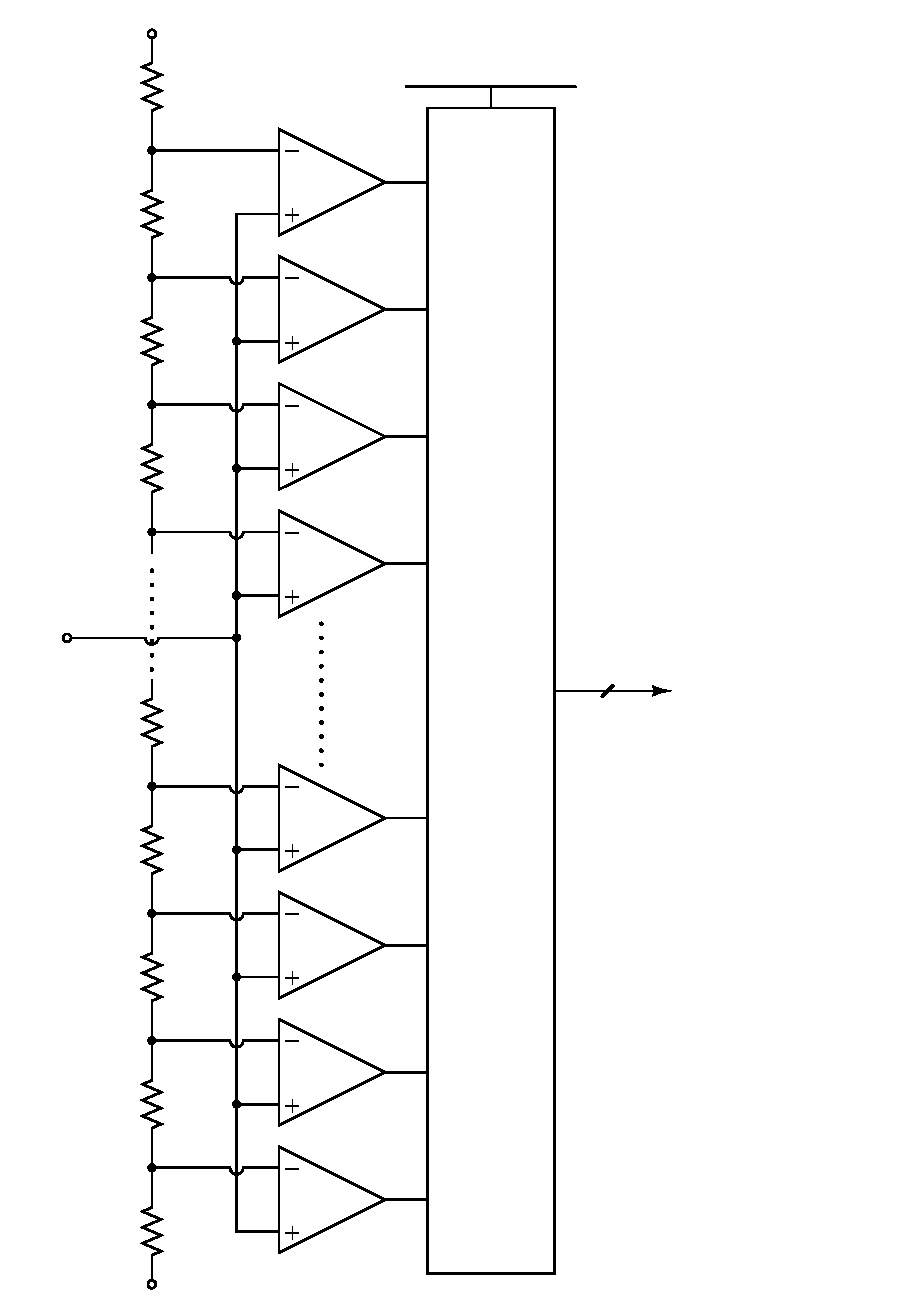
\includegraphics[width=0.9\textwidth]{./final_figures/Flash_ADC.eps}
 \caption{Flash ADC System Block Diagram}
 \label{fig:flash_adc}
\end{figure}
%-------------------

%%%%%%%%%%%%%%%%%%%%%%%%%%%%%%%%%%%%%%%%%%%%%%%%
%%% 2.4.1 Oversampling converters
%%%%%%%%%%%%%%%%%%%%%%%%%%%%%%%%%%%%%%%%%%%%%%%%
\subsection{Oversampling Converters}
Oversampling ADCs are ADCs which increase their effective resolution by
sampling their input signals at much higher rates than its Nyquist rate and
then band-limiting the quantization noise to the Nyquist bandwidth of the input signal.
The ratio of the sampling frequency, $f_s$, to the input signal's Nyquist rate, $2f_0$, is
referred to as the oversampling-rate (OSR) and in this thesis is denoted as $M$; that is, 
%---------------
\begin{equation}\label{eq:OSR}
 M=\frac{f_{s}}{2f_{0}}\text{.}
\end{equation}
%---------------

To illustrate, consider a Nyquist ADC with a sampling frequency, $f_s$, and an input
signal with a Nyquist bandwidth, $f_0$. As illustrated in Figure
\ref{fig:ADC_spectrum_comparison}(a), if $f_s=2f_0$, then the quantization noise is
uniformly distributed over the operational bandwidth, $f_\text{NY}$, where
$f_\text{NY}\in\left[-f_0,f_0\right]$. Alternatively, consider an oversampling ADC with a
sampling frequency, $f_s$, such that $f_s=M2f_0$ where $M$ is the OSR. For such an ADC,
the quantization noise is uniformly distributed over the operational bandwidth,
$f_{\text{OS}}$, where $f_\text{OS}\in \left[-f_s/2, f_s/2\right]$. As illustrated in
Figure \ref{fig:ADC_spectrum_comparison}(b), if the ADC's output is filtered so that it is
bandlimited to the input signal's Nyquist bandwidth, $f_0$, then the quantization noise
power distributed over the remaining frequencies, $f_0\leq\lvert f\rvert\leq Mf_0$, is
effectively removed from the output. Thus, the average quantization noise power is
decreased by a factor of $M$ and the SNR is increased by a factor of $M$ thereby
increasing the ADC's effective resolution. From observation of Figure
\ref{fig:ADC_spectrum_comparison}, the in-band quantization noise for the oversampling
converter is significantly less than the Nyquist converter.

To further illustrate, consider a $B$-bit oversampling ADC that has an OSR, $M$, with a
quantization noise power, $P_e$, that is uniformly distributed over its operational
bandwidth $\left[-f_s/2,f_s/2\right]$, where $f_s$ denotes the sampling frequency. If the
ADC's output is filtered so that the quantization noise power is bandlimited to the input
signal's Nyquist bandwidth, $\left[-f_0,f_0\right]$, the filtered output quantization
noise power, $P_{e,\text{OS}}$, can be expressed as
%---------------
\begin{equation}\label{eq:average_noise_power_only_OSR}
 P_{e,\text{OS}}=\frac{1}{f_s}\int_{-f_0}^{f_0}P_e
d f=P_e\frac{2f_0}{f_s}=\frac{P_e}{M}\text{.}
\end{equation}
%---------------
Thus, the average quantization noise power, $P_{e,\text{OS}}$, for an oversampling ADC
with an OSR, $M$, can be calculated by substituting \eqref{eq:quantization_noise_power}
into \eqref{eq:average_noise_power_only_OSR} which results in
%---------------
\begin{equation}\label{eq:average_noise_power_only_OSR_2}
 P_{e,\text{OS}}=\frac{\Delta^2}{12}\left(\frac{1}{M}\right)
\end{equation}
%---------------
where $\Delta$ corresponds to the quantization step size. Substituting
\eqref{eq:average_noise_power_only_OSR_2} into \eqref{eq:SNR} and solving for the
theoretical SNR for an oversampled Nyquist rate converter which is stimulated by a
full-scale sinusoid as defined by \eqref{eq:fs_sinusoid_power} yields
%---------------
\begin{equation}\label{eq:SNR_OSR}
\begin{split}
\text{SNR}_\text{dB,OS}& =
10\log\frac{\left(\displaystyle\frac{\Delta^22^{2B}}{8}\right)}{\left(\displaystyle\frac
{\Delta^2}{12M}\right)}\\
& =10\log\Bigl(2^{2B}\bigl(3/2\bigr)M\Bigr)\\
& = 6.02B + 1.76+10\log(M)
\end{split}
\end{equation}
%---------------
where $B$ is the number of quantization bits and $M$ is the OSR. Because the maximum OSR
is a function of the ADC's maximum sampling frequency, $M$ is typically selected between 8
and 256. As such, oversampling converters can typically achieve a 9 to 24 dB increase in
SNR which is equivalent to an increase of 1 to 3 bits in effective resolution.

%%%%%%%%%%%%%%%%%%%%%%%%%%%%%%%%%%%%%%%%%%%%%%%%
%%% 2.4.1 Delta Sigma Modulators
%%%%%%%%%%%%%%%%%%%%%%%%%%%%%%%%%%%%%%%%%%%%%%%%
\subsection[Delta Sigma Modulators]{$\Delta\Sigma$ Modulators}
$\Delta\Sigma$ modulators are an ADC architecture that uses oversampling and a feedback
loop to achieve high signal to noise ratios (SNRs) and large dynamic ranges (DRs). Because
of the simplicity of the architecture, $\Delta\Sigma$ modulators can be implemented
using relatively simple analog circuitry in standard CMOS processes which offer low-power
performance and high levels of integration for mixed-signal
electronics\cite{kester_analog_2006}.

To achieve a large DR and high SNR, $\Delta\Sigma$ modulators are designed so that the
quantization noise's feedback loop filter, or noise transfer function (NTF), attenuates
the quantization noise within the frequency band of interest. Additionally, as with other
oversampling ADCs, the $\Delta\Sigma$ modulator's output is bandlimited to the input
signal's Nyquist bandwidth, $f_0$. A comparison of the output spectra for a Nyquist rate
converter, an oversampling converter, and a $\Delta\Sigma$ modulator is shown in Figure
\ref{fig:ADC_spectrum_comparison} (adapted from \cite{kester_ADC_arch_2005}) which
illustrates the relative amount of in-band noise power for each architecture.
As illustrated in Figure \ref{fig:ADC_spectrum_comparison}(c), the amount of
in-band noise power for $\Delta\Sigma$ modulators is largely determined by the shape of
the NTF.
%-------------------
\begin{figure}[H]
 \centering
 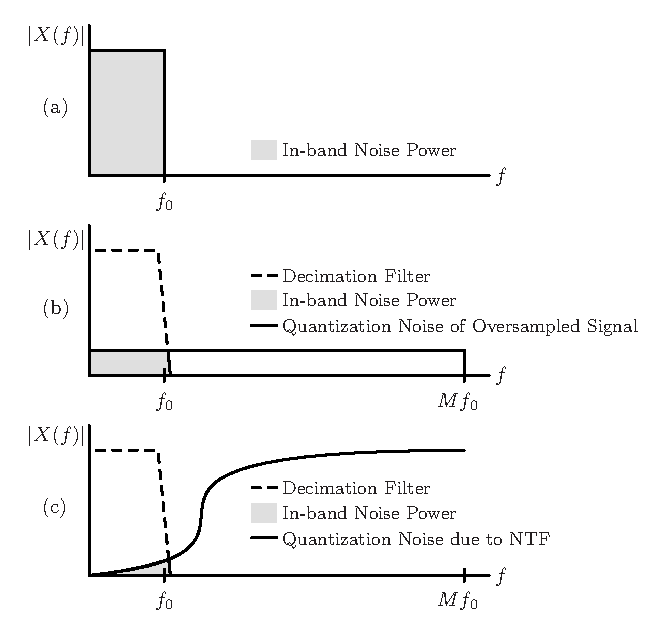
\includegraphics[width=0.8\textwidth]{./final_figures/ADC_spectrum_comparison}
\captionsetup{justification=centering} 
\caption[]{
ADC Output Noise Spectrum Comparison\\
(a) Nyquist Rate Converter 
(b) Oversampling Converter 
(c) $\Delta\Sigma$ Modulator
}
 \label{fig:ADC_spectrum_comparison}
\end{figure}
%-------------------

%%%%%%%%%%%%%%%%%%%%%%%%%%%%%%%%%%%%%%%%%%%%%%%%
%%% 2.4.1 Noise Shaping
%%%%%%%%%%%%%%%%%%%%%%%%%%%%%%%%%%%%%%%%%%%%%%%%
\subsubsection{Noise Shaping}
Figure \ref{fig:linear_block_diagram} illustrates a generic system structure of a
discrete-time $\Delta\Sigma$ modulator. The input block, $F(z)$, is a discrete system that
samples the analog input signal, $x_a(t)$, and processes the resulting discrete-time,
continuous amplitude signal, $x_a(n T_s)$. The ADC
block quantizes, or digitizes, $x_a(n T_s)$ to one of $2^B$ quantization levels, 
where $B$ denotes the number of bits in the digital output, $x(n)$. The
feedback DAC then converts the digital output signal, $x(n)$, into a discrete signal that
is fedback through $H(z)$ and into $G(z)$.
%-------------------
\begin{figure}[htbp]
	\centering
	\includegraphics{./final_figures/linear_block_diagram.eps}
	\caption{$\Delta\Sigma$ Modulator Block Diagram}
	\label{fig:linear_block_diagram}
\end{figure}
%-------------------

Figure \ref{fig:linear_simulation_model} illustrates Figure
\ref{fig:linear_block_diagram}'s generic \DS modulator where the ADC's quantizer is
modeled as an additive white noise source. For this thesis, only single-bit quantizers are
considered. As such, the time required for data conversion, or latency through the ADC and
the DAC, can be modeled as a unit delay in the feedback path.
 %-----------------------
\begin{figure}[htbp]
	\centering
	\includegraphics{./final_figures/linear_block_simulation.eps}
	\caption{$\Delta\Sigma$ Modulator Linear Model Block Diagram}
	\label{fig:linear_simulation_model}
\end{figure}
%-----------------------

Because the blocks, $F(z)$, $G(z)$, and $H(z)$ are typically implemented as linear time
invariant (LTI) subsystems, the NTF and STF can be expressed as 
%-----------------------
\begin{equation}\label{eq:STF}
\text{STF}(z)=\frac{Y(z)}{X(z)}=\frac{F(z)G(z)}{1+z^{-1}G(z)H(z)}
\end{equation}
%-----------------------
and
%-----------------------
\begin{equation}\label{eq:NTF}
\text{NTF}(z)=\frac{Y(z)}{E(z)}=\frac{1}{1+z^{-1}G(z)H(z)}\text{.}
\end{equation}
%-----------------------

Figure \ref{fig:DSM_loop_filters} illustrates a STF and NTF for a lowpass $\Delta\Sigma$
modulator where the quantization noise is attenuated by a highpass NTF and the input
signal is filtered by a lowpass STF.
%-----------------------
\begin{figure}[htbp]
	\centering
	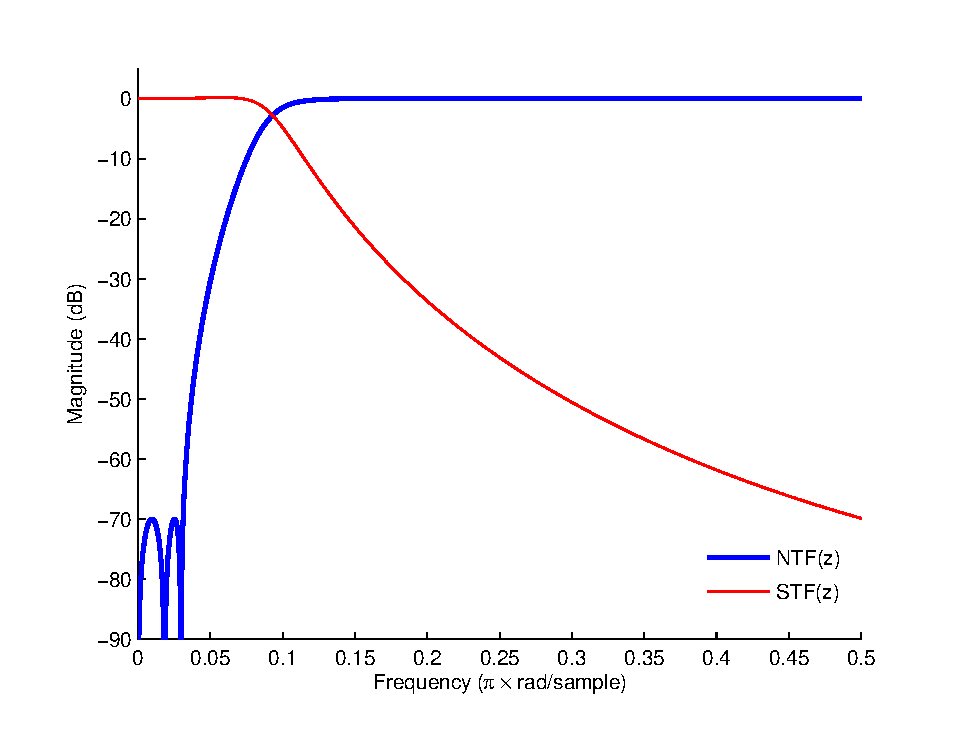
\includegraphics[width=0.65\textwidth]{./matlab_figures/LPDSM_spec_ex}
	\caption[Example: \DS Modulator Magnitude Response]{Examples of a STF and NTF
Magnitude Responses for a Lowpass Discrete-Time \DS Modulator}
	\label{fig:DSM_loop_filters}
\end{figure}
%-----------------------
If the NTF and STF are modeled as LTI systems, the output, $Y(z)$, of a \DS modulator can
be expressed as
%-----------------------
\begin{equation}\label{eq:DSM_output}
 Y(z)=\text{STF}(z)X(z)+\text{NTF}(z)E(z)
\end{equation}
%-----------------------
where $X(z)$ and $E(z)$ correspond to the $\mathcal{z}$-transforms of the input signal
and quantization noise respectively.

\subsection[Delta Sigma Modulator Implementations: Linear Models]
{$\Delta\Sigma$ Modulator Implementations: Linear Models}
The $\Delta\Sigma$ modulator that has been mathematically modeled by the block
diagram shown in Figure \ref{fig:linear_block_diagram} can be implemented using many
different structures. Common hardware implementations include
cascade-of-resonators-feedback (CRFB), cascade-of-resonators-feedforward (CRFF),
cascade-of-integrators-feedback (CIFB), and cascade-of-integrators-feedforward
\cite{schreier_understanding_2004}. For this thesis, a CRFB implementation was
implemented.

\subsubsection{First Order System}
\DS modulator implementations which utilize analog hardware (e.g. integrators) to realize
their loop filters are referred to as continuous-time $\Delta\Sigma$ modulators. For
example, Figure \ref{fig:ct_first_order} illustrates a 1st order, continuous-time \DS
modulator.
%-------------------
\begin{figure}[htbp]
 \centering
 \includegraphics{./final_figures/ct_dsm_model.eps}
 \caption{First-Order \CTDSM}
 \label{fig:ct_first_order}
\end{figure}
%-------------------
Similarly, implementations which utilize discrete-time hardware (e.g. accumulators) to
realize their loop filters  are referred to as discrete-time $\Delta\Sigma$ modulators. As
illustrated in Figures \ref{fig:ct_first_order} and \ref{fig:dt_first_order},
discrete-time \DS modulators typically use an accumulator in place of the
integrators.
%-------------------
\begin{figure}[htbp]
 \centering
 \includegraphics{./final_figures/dt_dsm_model.eps}
 \caption{First-Order \DTDSM}
 \label{fig:dt_first_order}
\end{figure}
%-------------------
Because discrete-time \DS modulators use discrete-time hardware to realize their loop
filters, traditional discrete-time design and analysis techniques can be used
\cite{hayes_schaums_1998}\cite{cherry_continuous-time_1999}.

Figure  \ref{fig:linear_z_model_1} shows a 1st order, discrete-time \DS modulator where 
the quantization noise is modeled as an additive white noise source. 
%-------------------
\begin{figure}[htbp]
 \centering
 \includegraphics{./final_figures/first_order_simple.eps}
 \caption{First Order Linear Model}
 \label{fig:linear_z_model_1}
\end{figure}
%-------------------
Recall that a $\Delta\Sigma$ modulator's output can be modeled as the sum of the
quantization error and the input signal. For lowpass architectures, the quantization error
is highpass filtered by the NTF and the input signal is lowpass filtered by the STF as
described by \eqref{eq:DSM_output}. From observation of Figure \ref{fig:linear_z_model_1},
the \DS modulator's output, $Y(z)$, is given as
%-------------------
\begin{equation}\label{eq:1st_lin_easy1}
 Y(z)=E(z)+A(z)
\end{equation}
%-------------------
where $A(z)$ is the accumulator output which is given as 
%-------------------
\begin{equation}\label{eq:1st_lin_easy2}
 A(z)=z^{-1}A(z)+X(z)-z^{-1}Y(z)\text{.}
\end{equation}
%-------------------
Substituting \eqref{eq:1st_lin_easy2} into \eqref{eq:1st_lin_easy1}, the output,
$Y(z)$, can be expressed as 
%-------------------
\begin{equation}\label{eq:1st_lin_easy3}
 \begin{split}
  Y(z) &= E(z)+z^{-1}A(z)+X(z)-z^{-1}Y(z)\\
       &= X(z)+E(z)-z^{-1}\bigl(Y(z)-A(z)\bigr)\\
       &= X(z)+\bigl(1-z^{-1}\bigr)E(z)\text{.}
 \end{split}
\end{equation}
%-------------------
Comparing \eqref{eq:1st_lin_easy3} and \eqref{eq:DSM_output}, it can be seen that
%-------------------
\begin{equation}\label{eq:first_order_STF}
   \text{STF}(z)=1
\end{equation}
%-------------------
and
%-------------------
\begin{equation}\label{eq:first_order_NTF}
   \text{NTF}(z)=\left(1-z^{-1}\right)
\end{equation}
%-------------------
which implies that the input signal, $X(z)$, is unaltered at the output and the
quantization noise, $E(z)$, is lowpass filtered by the first order expression
$\left(1-z^{-1}\right)$.

The location of the poles and zeros of the NTF and STF determine the
characteristics of the NTF's and STF's frequency response. However, the \DS modulator
shown in Figure \ref{fig:linear_z_model_1} does not allow the pole and zero locations to
be adjusted. The pole locations can be adjusted by adding feedback
coefficients to the \DS modulator as illustrated in Figure \ref{fig:linear_z_model_2}.
%-------------------
\begin{figure}[htbp]
 \centering
 \includegraphics{./final_figures/first_order_linear_model.eps}
 \caption{Generalized First Order Linear Model}
 \label{fig:linear_z_model_2}
\end{figure}
%-------------------
From observation of Figure \ref{fig:linear_z_model_2}, the \DS
modulator's output, $Y(z)$, is given as
%-------------------
\begin{equation}\label{eq:1st_lin_1}
 Y(z)=E(z)+A(z)-\beta_{1}z^{-1}Y(z)
\end{equation}
%-------------------
where $A(z)$ is the accumulator output which is given as 
%-------------------
\begin{equation}\label{eq:1st_lin_2}
 \begin{split}
 A(z)& = z^{-1}A(z)+X(z)-\beta_{0}z^{-1}Y(z)\\
      &   = \frac{X(z)-\beta_{0}z^{-1}Y(z)}{\left(1-z^{-1}\right)}\text{.}
 \end{split}
\end{equation}
%-------------------
Substituting \eqref{eq:1st_lin_2} into \eqref{eq:1st_lin_1} the output,
$Y(z)$, can be expressed as 
%-------------------
\begin{equation}\label{eq:1st_lin_3}
  \begin{split}
  Y(z)& =
E(z)+\frac{X(z)-\beta_{0}z^{-1}Y(z)}{\left(1-z^{-1}\right)}-\beta_{1}z^{-1}Y(z)\\
        & =
\frac{\bigl(1-z^{-1}\bigr)E(z)+X(z)}{\Bigl(1+\bigl(\beta_{0}+\beta_{1}-1\bigr)z^{-1}
-\beta_{1}z^{-2}\Bigr)}\\
     & = \frac{X(z)}{\Bigl(1+\bigl(\beta_{0}+\beta_{1}-1\bigr)z^
{-1}-\beta_{1}z^{-2}\Bigr)}+\frac{\bigl(1-z^{-1}\bigr)E(z)}{\Bigl(1+\bigl(\beta_{0}
 +\beta_{1}-1\bigr)z^{-1}-\beta_{1}z^{-2}\Bigr)}\text{.}
 \end{split}
\end{equation}
%-------------------
Comparing \eqref{eq:1st_lin_3} and \eqref{eq:DSM_output}, it can be seen that
%-------------------
\begin{equation}\label{eq:1st_lin_STF}
   \text{STF}(z)=
\frac{1}{\Bigl(1+\bigl(\beta_{0}+\beta_{1}-1\bigr)z^{-1}-\beta_{1}z^{-2}\Bigr)}
\end{equation}
%-------------------
and
%-------------------
\begin{equation}\label{eq:1st_lin_NTF}
 \text{NTF}(z)=
	\frac{\bigl(1-z^{-1}\bigr)}{\Bigl(1+\bigl(\beta_{0}+\beta_{1}-1\bigr)z^{-1}-
	\beta_{1}z^{-2}\Bigr)}\text{.}
\end{equation}
%-------------------
For most applications, $\beta_1=0$. For such applications the transfer
functions described by \eqref{eq:1st_lin_STF} and \eqref{eq:1st_lin_NTF} can be
written as
%-------------------
\begin{equation}\label{eq:1st_lin_STF_reduced}
   \text{STF}(z)=
\frac{1}{1+\left(\beta_{0}-1\right)z^{-1}}
\end{equation}
%-------------------
and
%-------------------
\begin{equation}\label{eq:1st_lin_NTF_reduced}
 \text{NTF}(z)=
	\frac{\left(1-z^{-1}\right)}{1+\left(\beta_{0}-1\right)z^{-1}}
\end{equation}
%-------------------
respectively. Thus, \eqref{eq:1st_lin_STF_reduced} and \eqref{eq:1st_lin_NTF_reduced} are
equivalent to \eqref{eq:first_order_STF} and \eqref{eq:first_order_NTF} when $\beta_0=1$.

%%%%%%%%%%%%%%%%%%%%%%%%%%%%%%%%%%%%%%%%%%%%%%%%%%%%%%%%%%%%%%%%%%%%%%%%%%%%%%%%
\subsubsection{Second Order System}
Because the NTFs of 1st order $\Delta\Sigma$ modulators have a limited amount of
quantization noise attenuation, higher order systems are generally used. Consider the
second order system illustrated in Figure \ref{fig:linear_z_model_2nd_order}. This
system can be formed by cascading two first order systems together. 
%-------------------
\begin{figure}
  \centering
  \includegraphics[width=\textwidth]{./final_figures/second_order_simple_model.eps}
  \caption{Second Order Linear Model}
  \label{fig:linear_z_model_2nd_order}
\end{figure}
%-------------------
From observation of Figure \ref{fig:linear_z_model_2nd_order}, the second order \DS
modulator's output, $Y(z)$, is given
as
%-------------------
\begin{equation}\label{eq:2nd_order_DSM_output_1}
 Y(z)=E(z)+A_1(z)
\end{equation}
%-------------------
where $A_1(z)$ corresponds to the output of the second accumulator. The accumulator
outputs, $A_{0}$ and $A_{1}$, can be expressed as
%-------------------
\begin{equation}\label{eq:2nd_order_DSM_accumulator_0}
  A_{0}(z) = \frac{X(z)-z^{-1}Y(z)}{1-z^{-1}}
 \end{equation}
 %-------------------
and
%-------------------
\begin{equation}\label{eq:2nd_order_DSM_accumulator_1}
  A_{1}(z) = \frac{A_{0}(z)-z^{-1}Y(z)}{1-z^{-1}}\text{.}
\end{equation}
%-------------------
Substituting \eqref{eq:2nd_order_DSM_accumulator_0} into
\eqref{eq:2nd_order_DSM_accumulator_1} and the result into
\eqref{eq:2nd_order_DSM_output_1}, the
output, $Y(z)$, can be expressed as 
%-------------------
\begin{equation}\label{eq:2nd_order_DSM_output}
  Y(z) = X(z)+ \bigl(1-z^{-1}\bigr)^2 E(z)\text{.}
\end{equation}
%-------------------
Comparing \eqref{eq:2nd_order_DSM_output} and \eqref{eq:DSM_output}, it can be seen that
%-------------------
\begin{equation}\label{eq:second_order_STF}
   \text{STF}(z)=1
\end{equation}
%-------------------
and
%-------------------
\begin{equation}\label{eq:second_order_NTF}
   \text{NTF}(z)=\left(1-z^{-1}\right)^2
\end{equation}
%-------------------
which implies that the input signal, $X(z)$, is unaltered at the output and the
quantization noise, $E(z)$, is lowpass filtered by the second order expression
$\left(1-z^{-1}\right)^2$.

To adjust the pole locations of the 2nd order \DS modulator shown in Figure
\ref{fig:linear_z_model_2nd_order} feedback coefficients, denoted as $\beta_0$, $\beta_1$,
 and $\beta_2$, can be added as shown in Figure
\ref{fig:linear_z_model_2nd_order_complex}. 
%-------------------
\begin{figure}
  \centering
  \includegraphics[width=\textwidth]{./final_figures/second_order_complex_model.eps}
  \caption{Generalized Second Order Linear Model}
  \label{fig:linear_z_model_2nd_order_complex}
\end{figure}
%-------------------
From observation of Figure \ref{fig:linear_z_model_2nd_order_complex}, the \DS
modulators's output, $Y(z)$, is given as 
%-------------------
\begin{equation}\label{eq:2nd_order_DSM_output_complex_1}
 Y(z) = E(z)+A_1(z)-\beta_2 z^{-1}Y(z)
\end{equation}
%-------------------
where $A_1(z)$ corresponds to the output of the second accumulator. The accumulator
outputs, $A_{0}$ and $A_{1}$, can be expressed as
%-------------------
\begin{equation}\label{eq:2nd_order_DSM_accumulator_0_complex}
  A_{0}(z) = \frac{X(z)-\beta_0 z^{-1}Y(z)}{1-z^{-1}} 
\end{equation}
%-------------------
and
%-------------------
\begin{equation}\label{eq:2nd_order_DSM_accumulator_1_complex}
  A_{1}(z) = \frac{A_{0}(z)-\beta_1 z^{-1}Y(z)}{1-z^{-1}}=\frac{X(z)-(\beta_0+\beta_1)
z^{-1}Y(z)}{\left(1-z^{-1}\right)^2}
\end{equation}
%-------------------
Substituting \eqref{eq:2nd_order_DSM_accumulator_0_complex} into 
\eqref{eq:2nd_order_DSM_accumulator_1_complex} and the result into 
\eqref{eq:2nd_order_DSM_output_complex_1}, the
output, $Y(z)$, can be expressed as 
%-------------------
\begin{equation}\label{eq:2nd_order_DSM_output_complex}
 \begin{split}
  Y(z)& = E(z)+\frac{X(z)-(\beta_0+\beta_1)
z^{-1}Y(z)}{\left(1-z^{-1}\right)^2}-\beta_2 z^{-1}Y(z) \\
       & = \frac{X(z)+ \bigl(1-z^{-1}\bigr)^2 E(z)}
{ 1+ z^{-1}\bigl(-2+\beta_0+\beta_1+\beta_2\bigr)
   + z^{-2}\bigl(1-\beta_1-2\beta_2\bigr)
   + z^{-3}\beta_2}.\\
 \end{split}
\end{equation}
%-------------------
Comparing \eqref{eq:2nd_order_DSM_output_complex} and \eqref{eq:DSM_output}, it can be
seen that
%-------------------
\begin{equation}\label{eq:second_order_STF_complex}
   \text{STF}(z)= \frac{1}{
  1+ z^{-1}\bigl(-2+\beta_0+\beta_1+\beta_2\bigr)
   + z^{-2}\bigl(1-\beta_1-2\beta_2\bigr)
   + z^{-3}\beta_2}
\end{equation}
%-------------------
and
%-------------------
\begin{equation}\label{eq:second_order_NTF_complex}
   \text{NTF}(z)=\frac{\bigl(1-z^{-1}\bigr)^2 }{
  1+ z^{-1}\bigl(-2+\beta_0+\beta_1+\beta_2\bigr)
   + z^{-2}\bigl(1-\beta_1-2\beta_2\bigr)
   + z^{-3}\beta_2}\text{.}
\end{equation}
%-------------------

For most applications, $\beta_2=0$. For such applications the transfer functions
described by \eqref{eq:second_order_STF_complex} and
\eqref{eq:second_order_NTF_complex}) can be written as
%-------------------
\begin{equation}\label{eq:2nd_lin_STF_reduced}
   \text{STF}(z)= \frac{1}{
  1+ z^{-1}\bigl(-2+\beta_0+\beta_1\bigr)
   + z^{-2}\bigl(1-\beta_1\bigr)}
\end{equation}
%-------------------
and
%-------------------
\begin{equation}\label{eq:2nd_lin_NTF_reduced}
   \text{NTF}(z)=\frac{\left(1-z^{-1}\right)^2 }{
  1+ z^{-1}\bigl(-2+\beta_0+\beta_1\bigr)
   + z^{-2}\bigl(1-\beta_1\bigr)}
\end{equation}
%-------------------
respectively. Thus, \eqref{eq:2nd_lin_STF_reduced} and
\eqref{eq:2nd_lin_NTF_reduced} are
equivalent to \eqref{eq:second_order_STF} and \eqref{eq:second_order_NTF} when
$\beta_0=\beta_1=1$.

Because a \DS modulator's NTF is designed first, the feedback coefficients,
$\{\beta_n\}$, 
are chosen to optimize the NTF's characteristics. As such, the STFs in
\eqref{eq:second_order_STF_complex} and \eqref{eq:2nd_lin_STF_reduced} are fixed by the
NTF's design. To shape the STF, feedforward coefficients can be added to Figure
\ref{fig:linear_z_model_2nd_order_complex} as illustrated in Figure
\ref{fig:general_2nd_order}.
%-------------------
\begin{figure}
  \centering
  \includegraphics[width=\textwidth]{./final_figures/general_2nd_order.eps}
  \caption[Second Order Linear Model with Feedforward Coefficients]{Generalized Second
Order Linear Model with Feedforward Coefficients}
  \label{fig:general_2nd_order}
\end{figure}
%-------------------
From observation of Figure \ref{fig:general_2nd_order}, the \DS modulator's output,
$Y(z)$, is given as 
%-------------------
\begin{equation}\label{eq:2nd_order_DSM_output_general}
 Y(z)=E(z)+\alpha_2 X(z)+A_1(z)-\beta_2 z^{-1}Y(z)
\end{equation}
%-------------------
where $A_1(z)$ corresponds to the output of the second accumulator. The accumulator
outputs, $A_{0}$ and $A_{1}$, can be expressed as
%-------------------
\begin{equation}\label{eq:2nd_order_DSM_accumulator_0_general}
  A_{0}(z) = \frac{\alpha_0 X(z)-\beta_0 z^{-1}Y(z)}{1-z^{-1}} 
\end{equation}
%-------------------
and
%-------------------
\begin{equation}\label{eq:2nd_order_DSM_accumulator_1_general}
  A_{1}(z) = \frac{\alpha_1 X(z)+ A_{0}(z)-\beta_1 z^{-1}Y(z)}{1-z^{-1}}\text{.}
\end{equation}
%-------------------
Substituting \eqref{eq:2nd_order_DSM_accumulator_0_general} into
\eqref{eq:2nd_order_DSM_accumulator_1_general} and the result into
\eqref{eq:2nd_order_DSM_output_general}, the
output, $Y(z)$, can be expressed as 
%-------------------
\begin{equation}\label{eq:2nd_order_DSM_output_general_2}
\begin{split}
 Y(z)& =\left(\frac{
\bigl(\alpha_0+\alpha_1+\alpha_2\bigr)-z^{-1}\bigl(\alpha_1+2\alpha_2\bigr)+z^{-2}\alpha_2
}
{  1+ z^{-1}\bigl(-2+\beta_0+\beta_1+\beta_2\bigr)
   + z^{-2}\bigl(1-\beta_1-2\beta_2\bigr)
   + z^{-3}\beta_2}\right) X(z)\\
&\quad + \left(\frac{\bigl(1-z^{-1}\bigr)^2}
{  1+ z^{-1}\bigl(-2+\beta_0+\beta_1+\beta_2\bigr)
   + z^{-2}\bigl(1-\beta_1-2\beta_2\bigr)
   + z^{-3}\beta_2}\right)E(z)\text{.}
\end{split}
\end{equation}
%-------------------
Comparing \eqref{eq:2nd_order_DSM_output_general_2} and \eqref{eq:DSM_output}, it can
be seen that
%-------------------
\begin{equation}\label{eq:second_order_STF_general_2_STF}
   \text{STF}(z)= \frac{
\bigl(\alpha_0+\alpha_1+\alpha_2\bigr)-z^{-1}\bigl(\alpha_1+2\alpha_2\bigr)+z^{-2}\alpha_2
}
{  1+ z^{-1}\bigl(-2+\beta_0+\beta_1+\beta_2\bigr)
   + z^{-2}\bigl(1-\beta_1-2\beta_2\bigr)
   + z^{-3}\beta_2}
\end{equation}
%-------------------
and
%-------------------
\begin{equation}\label{eq:second_order_STF_general_2_NTF}
   \text{NTF}(z)=
\frac{\bigl(1-z^{-1}\bigr)^2}
{  1+ z^{-1}\bigl(-2+\beta_0+\beta_1+\beta_2\bigr)
   + z^{-2}\bigl(1-\beta_1-2\beta_2\bigr)
   + z^{-3}\beta_2}\text{.}
\end{equation}
%-------------------
It can be observed from \eqref{eq:second_order_STF_general_2_STF} and
\eqref{eq:second_order_STF_general_2_NTF} that the feedforward coefficients, $\alpha_0$,
$\alpha_1$, and $\alpha_2$, only affect the STF and not the NTF. As such, this allows the
shape of the STF to be
changed independently from the NTF. It also can be seen that
\eqref{eq:second_order_STF_general_2_STF} and \eqref{eq:second_order_STF_general_2_NTF}
are equivalent to
\eqref{eq:second_order_STF_complex} and \eqref{eq:second_order_NTF_complex} for
$\alpha_1=\alpha_2=0$ and $\alpha_0=1$.

\subsubsection{High Order Systems}
Theoretically, a \DS modulator's order, $n$, has no upper bound and thus, the NTF's
stopband attenuation can be increased to any arbitrarily large level. This in turn would
allow the effective resolution of the \DS modulator to increase without bound. However,
physical phenomena such as thermal noise and clock jitter typically limit a \DS
modulator's achievable effective resolution. Therefore, in practice, $\Delta\Sigma$
modulators are typically designed such that $n\leq8$. 

Additionally, because the internal voltage swings of a \DS modulator are limited by the
electrical characteristics of its process technology, scaling coefficients are
typically placed between adjacent integrators to avoid saturation. Saturation, or
clipping, can cause instability and introduces nonlinear distortion thereby decreasing
the effective resolution of the $\Delta\Sigma$ modulator. Figure
\ref{fig:linear_z_model_nth_order} illustrates a generalized $n$th order converter
topology with scaling coefficients, denoted $c_x$, between adjacent integrators where $x$
corresponds to the coefficient's respective integrator number.
%-------------------
\begin{sidewaysfigure}[htbp]
  \centering
  \includegraphics[width=\textwidth]{./final_figures/general_nth_order_2.eps}
  \caption{Generalized $n$th Order Linear Model}
  \label{fig:linear_z_model_nth_order}
\end{sidewaysfigure}
%-------------------

%%%%%%%%%%%%%%%%%%%%%%%%%%%%%%%%%%%%%%%%%%%%%%%%
%%% 2.4.5 DSM Theoretical Performance
%%%%%%%%%%%%%%%%%%%%%%%%%%%%%%%%%%%%%%%%%%%%%%%%
\subsection[Delta Sigma Modulator Theoretical Performance]
{$\Delta\Sigma$ Modulator Theoretical Performance}
The theoretical effective resolution of a \DS modulator can be calculated if the shape of
in-band NTF is known. That is, stochastic system theory can be used to predict the
performance of a deterministic system function for a particular input, $x(n)$, and
the randomly modeled quantization noise, $q(n)$. 

Stochastic system theory states that for an LTI system, an input signal, $x(n)$, which
can be modeled as a discrete-time random process, will produce an output
signal, $y(n)$, which can also be modeled as a discrete-time random
process\cite{papoulis_probability_1984}. As such, descriptive statistics (e.g. mean,
variance, and autocorrelation) are often used to analyze LTI system's output signals when
the input signals can be modeled as random processes.

The autocorrelation, $R_{x(n)}(k)$, of a discrete-time random process, $x(n)$,
can be expressed as
%----------------------
\begin{equation}\label{eq:autocorrelation}
 R_{x(n)}(k)=E\left[x(n)x(n+k)\right]
\end{equation}
%----------------------
where $E[\cdot]$ denotes the expectation operator as defined in
\eqref{eq:discrete_ensemble_average}\cite{hsu_schaums_1996}. If $x(n)$ is a zero mean,
random process then the autocorrelation of $x(n)$ for $k=0$, $R_{x(n)}(0)$, is equivalent
to the variance, $\sigma^2_{x(n)}$, of $x(n)$, as described by
\eqref{eq:expectation_proof}; that is,
%----------------------
\begin{equation}\label{eq:autocorrelation_zero_1}
 R_{x(n)}(0)=E\left[x(n)x(n+0)\right]=E\left[x^2(n)\right]=\sigma^2_{x(n)}\text{.}
\end{equation}
%----------------------
As such, the average power, $P_{x(n)}$, of a zero mean, random process, $x(n)$, can be
expressed as 
%----------------------
\begin{equation}\label{eq:autocorrelation_zero_2}
 P_{x(n)}=R_{x(n)}(0)\text{.}
\end{equation}
%----------------------

It has been shown \cite{oppenheim_discrete-time_1999} that the power spectral
density, $\bm{S}_{x(n)}(e^{j\omega})$, of a discrete-time random process,
$x(n)$, can be calculated by taking the Fourier transform of its autocorrelation,
$R_{x(n)}(k)$; that is,
%----------------------
\begin{equation}\label{eq:power_spectrum}
 \bm{S}_{x(n)}(e^{j\omega})=\sum_{k=-\infty}^{\infty}{R_{x(n)}(k)e^{
-j\omega k}}
\end{equation}
%----------------------
where $\omega$ denotes frequency in radians per sample. Conversely, the autocorrelation of
a discrete-time random process, $R_{x(n)}(k)$, can be calculated by taking the inverse
Fourier transform of its power spectral density, $\bm{S}_{x(n)}(e^{j\omega})$, which
implies that 
%----------------------
\begin{equation}\label{eq:autocorrelation_psd}
 R_{x(n)}(k)=\frac{1}{2\pi}\int_{-\pi}^{\pi}{\bm{S}_{x(n)}(e^{j\omega})
e^{j\omega k} d\omega} \text{.}
\end{equation}
%----------------------
It has also been shown \cite{hsu_schaums_1996}\cite{oppenheim_discrete-time_1999} that
the output power spectral density, $\bm{S}_{y(n)}(e^{j\omega})$, of a LTI
system that has a frequency response, $H(e^{j\omega})$, can be calculated by
taking the product of the input power spectral density,
$\bm{S}_{x(n)}(e^{j\omega})$, and the magnitude-squared of the
system's frequency response; that is, 
%----------------------
\begin{equation}\label{eq:LTI_psd}
 \bm{S}_{y(n)}(e^{j\omega})=\lvert
H(e^{j\omega})\rvert^2\bm{S}_{x(n)}(e^{j\omega})\text{.}
\end{equation}
%----------------------
Therefore using \eqref{eq:autocorrelation_psd} and \eqref{eq:LTI_psd}, the
autocorrelation,
$R_{y(n)}(k)$, of the output, $y(n)$, of an LTI system that has the input $x(n)$ can be
written as
%----------------------
\begin{equation}\label{eq:LTI_output_autocorrelation}
\begin{split}
R_{y(n)}(k)& =\frac{1}{2\pi}\int_{-\pi}^{\pi}\bm{S}_{y(n)}(e^{j\omega})e^{
j\omega k} d\omega\\
& = \frac{1}{2\pi}\int_{-\pi}^{\pi}
\lvert H(e^{j\omega})\rvert^2\bm{S}_{x(n)}(e^{j\omega})e^{
j\omega k} d\omega.
\end{split}
\end{equation}
%----------------------
Using \eqref{eq:autocorrelation_zero_2} and \eqref{eq:LTI_output_autocorrelation}, the
average output power, $P_{y(n)}$, of an LTI system can be calculated as
%----------------------
\begin{equation}\label{eq:LTI_average_output_power}
P_{y(n)}=R_{y(n)}(0)=\frac{1}{2\pi}\int_{-\pi}^{\pi}
\lvert
H(e^{j\omega})\rvert^2\bm{S}_{x(n)}(e^{j\omega})d\omega\text{.}
\end{equation}
%----------------------

Because a \DS modulator's NTF is modeled as a LTI system, its output quantization noise
power, $P_{q(n)}$, can be calculated using \eqref{eq:LTI_average_output_power}; that is,
%---------------
\begin{equation}\label{eq:average_noise_power_NTF}
 P_{q(n)}=\frac{1}{2\pi}\int_{-\omega_0}^{\omega_0}{\lvert
\text{NTF}(e^{j\omega})\rvert^2\bm{S}_{e(n)}(e^{j\omega})d\omega}
\end{equation}
%---------------
where $\omega_0$ corresponds to the Nyquist frequency of the input signal in radians per
sample.

To determine the quantization noise power spectral density, $\bm{S}_{e(n)}(e^{j\omega})$,
the quantization noise is assumed to be a zero mean, uncorrelated white noise process,
which implies that its autocorrelation, $R_{e(n)}(k)$, can be written as
%---------------
\begin{equation}\label{eq:quantization_noise_psd_2}
R_{e(n)}(k)=E\left[e(n)e(n+k)\right]=E\left[e^2(n)\right]\delta(k)=\sigma^2_{e(n)}
\delta(k).
\end{equation}
%---------------
Therefore, the power spectral density of the quantization noise,
$\bm{S}_{e(n)}(e^{j\omega})$, can be written as
%---------------
\begin{equation}\label{eq:quantization_noise_psd_3}
\bm{S}_{e(n)}(e^{j\omega})=\sum_{k=-\infty}^{\infty}\sigma^2_{e(n)}
\delta(k)e^{-j\omega k}=\sigma^2_{e(n)}=P_{e(n)}.
\end{equation}
%---------------
Thus, substituting \eqref{eq:quantization_noise_power} into
\eqref{eq:quantization_noise_psd_3}, it can be seen that 
%---------------
\begin{equation}\label{eq:quantization_noise_psd_6}
\bm{S}_{e(n)}(e^{j\omega})=\frac{\Delta^2}{12}
\end{equation}
%---------------
where $\Delta$ is the quantization interval. Substituting
\eqref{eq:quantization_noise_psd_6} into \eqref{eq:average_noise_power_NTF}, the  \DS
modulator's output quantization noise power, $P_{q(n)}$, can be expressed as
%---------------
\begin{equation}\label{eq:average_noise_power_NTF_2}
\begin{split}
P_{q(n)}& = \frac{1}{2\pi}\int_{-\omega_0}^{\omega_0}{
\lvert
\NTF(e^{j\omega})\rvert^2\bm{S}_{e(n)}(e^{j\omega})d\omega}\\
&
=\frac{1}{2\pi}\left(\frac{\Delta^2}{12}\right)\int_{-\omega_0}^{\omega_0}{
\lvert\NTF(e^{j\omega})\rvert^2d\omega}
\end{split}
\end{equation}
%---------------
where $\omega_0$ corresponds to the input signal's Nyquist bandwidth.

For the $n$th order discrete-time \DS modulator architecture shown in Figure
\ref{fig:linear_z_model_nth_order} where $a_n=b_n=c_n=1$, the NTF can be written as 
%---------------
\begin{equation}\label{eq:NTF_simple_z}
\NTF(z)=(1-z^{-1})^n
\end{equation}
%---------------
which implies that 
%---------------
\begin{equation}\label{eq:NTF_simple_jw}
\NTF(e^{j\omega})=(1-e^{-j\omega})^n=\Biggl(j2e^{-j\frac{\omega}{2}}
\left(\frac{e^{j\frac{\omega}{2}}-e^{-j\frac{\omega}{2}}}{j2}\right)\Biggr)^n.
\end{equation}
%---------------
Using Euler's identity\cite{thomas_thomas_2004}, \eqref{eq:NTF_simple_jw} can be written
as
%---------------
\begin{equation}\label{eq:NTF_simple_euler}
\NTF(e^{j\omega})=\biggl(j2e^{-j\frac{\omega}{2}}\sin\left(\frac{\omega}{2}
\right)\biggr)^n.
\end{equation}
%---------------
Thus, 
%---------------
\begin{equation}\label{eq:NTF_simple_magnitude}
\lvert \NTF(e^{j\omega})\rvert^2=\biggl\lvert
\biggl(j2e^{-j\frac{\omega}{2}}\sin\left(\frac{\omega}{2}
\right)\biggr)^n \biggr\rvert^2 = \biggl(2\sin\left(\frac{\omega}{2}\right)\biggr)^{2n}.
\end{equation}
%---------------
Substituting \eqref{eq:NTF_simple_magnitude} into \eqref{eq:average_noise_power_NTF_2},
the quantization noise power, $P_{q(n)}$, can be written as
%---------------
\begin{equation}\label{eq:quantization_power_some_more_fun}
P_{q(n)}=\frac{1}{2\pi}\left(\frac{\Delta^2}{12}\right)
\int_{-\omega_0}^{\omega_0}\biggl(2\sin\left(\frac{\omega}{2}\right)\biggr)^{2n}
d\omega.
\end{equation}
%---------------
For large OSRs, $\omega_0\ll\pi$, and therefore,
$$\sin\left(\frac{\omega}{2}\right)\approx\frac{\omega}{2}.$$
\cite{schreier_understanding_2004}\cite{thomas_thomas_2004}\cite{kozak_oversampled_2003}.
Substituting this approximation into \eqref{eq:quantization_power_some_more_fun}, the
output quantization noise power, $P_{q(n)}$, can be given as 
%---------------
\begin{equation}\label{eq:average_noise_power_NTF_3}
\begin{split}
P_{q(n)}&
=\frac{1}{2\pi}\left(\frac{\Delta^2}{12}\right)\int_{-\omega_0}^{\omega_0}\omega^{2n}
d\omega\\
& =
\frac{1}{2\pi}\left(\frac{\Delta^2}{12}\right)\left(\frac{\omega^{2n+1}}{2n+1}\biggl\vert_
{-\omega_0 }^{ \omega_0}\right)\\
&
=\frac{\Delta^2}{12\pi}\left(\frac{1}{2n+1}\right)\omega_0^{2n+1}.
\end{split}
\end{equation}
%---------------
Substituting $\omega_0=\pi/M$ into \eqref{eq:average_noise_power_NTF_3}, the
output quantization noise power, $P_{q(n)}$, can be expressed as
%---------------
\begin{equation}\label{eq:average_noise_power_NTF_4}
P_{q(n)}=\frac{\Delta^2}{12\pi}\left(\frac{1}{2n+1}\right)
\left(\frac{\pi}{M}\right)^{2n+1}
\end{equation}
%---------------
where $M$ denotes the OSR.

The theoretical $\text{SNR}_{\text{dB}}$, $\text{SNR}_\text{dB,LPDSM}$, for a lowpass
$\Delta\Sigma$ modulator that has a full-scale sinusoidal input as defined by
\eqref{eq:fs_sinusoid_power}, can be derived by substituting
\eqref{eq:average_noise_power_NTF_4} into \eqref{eq:SNR} such that
%---------------
\begin{equation}\label{eq:SNR_DSM}
\begin{split}
\text{SNR}_\text{dB,LPDSM}& =
10\log\frac{\left(\displaystyle\frac{\Delta^22^{2B}}{8}\right)}
{\displaystyle\frac{\Delta^2}{12\pi}\left(\frac{1}{2n+1}\right)
    \left(\frac{\pi}{M}\right)^{2n+1}}\\
&
=10\log\left(\frac{3}{2}2^{2B}
\right)+10\log\left(2n+1\right)-2n10\log(\pi)+(2n+1)10\log (M)
\\
& = 6.02B + 10\log(2n+1) - 20n\log(\pi)+(20n+10)\log(M)
\end{split}
\end{equation}
%---------------
where $M$ corresponds to the OSR and $B$ corresponds to the number of quantization
bits.
 
From observation of \eqref{eq:SNR_DSM}, it can be seen that the dominant term, that is the
term which has the greatest impact on SNR, in \eqref{eq:SNR_DSM} is $(20n+10)\log(M)$ for
$M\gg1$ which implies that the effective resolution for a $\Delta\Sigma$ modulator is
largely determined by the OSR and the order of the loop filter.